\documentclass[a4paper]{article}

\usepackage[T1]{fontenc}
\usepackage[utf8]{inputenc}
\usepackage[polish]{babel}
\usepackage{graphicx}
\graphicspath{{.}}

\usepackage[left = 2cm, right = 2cm, top = 2cm, bottom = 2cm] {geometry}

\usepackage{amsmath, amsfonts}
\usepackage{textcomp}

\pagestyle{empty}

\author{}
\title{}
\date{\today}

\begin{document}
\section*{Instrukcja gry "Monopoly UWr"}

%\paragraph*{Informacje ogólne}
\noindent \textbf{1.Informacje ogólne}\\
\noindent Gra przeznaczona jest dla 4 graczy. Mogą nimi być również zawarte w grze boty.
\vspace{10pt}

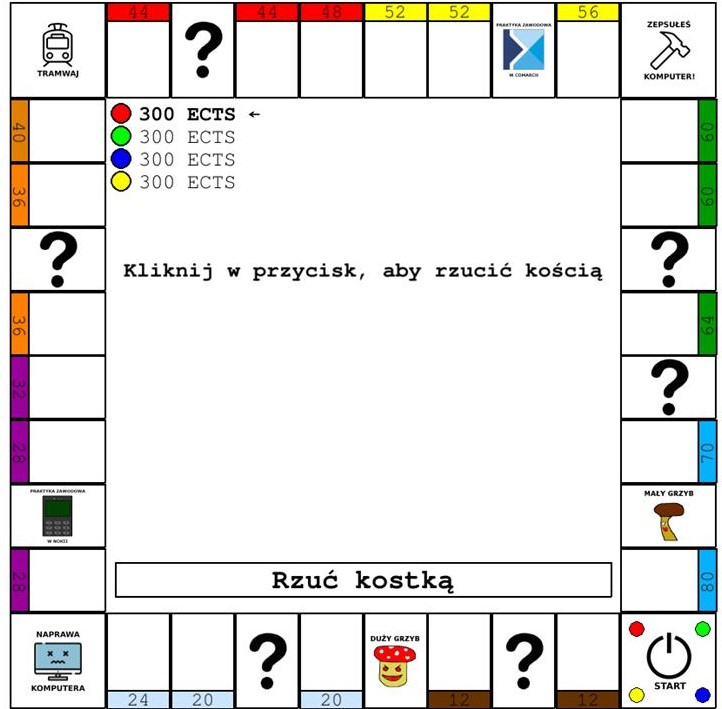
\includegraphics[scale=0.8]{board.png}

\noindent \textbf{2.Cel gry}\\
\noindent Celem jest zapisanie się i zaliczenie przedmiotów w czterech zakładach lub doprowadzenie pozostałych graczy do utraty wszystkich punktów.
\vspace{10pt}

%\paragraph*{Rozgrywka}
\noindent \textbf{3.Rozgrywka}\\
\noindent Wszyscy gracze rozpoczynają rozgrywkę na polu 'start'. Pionki graczy reprezentowane są przez kolorowe kółka. Tura gracza składa się z następujących akcji:\\
- rzut dwoma kostkami,\\
- przesunięcie swojego pionka o liczbę pól równą sumie wyrzuconych oczek w kierunku zgodnym z ruchem wskazówek zegara,\\
- wykonanie instrukcji zgodnie z opisem pola, na który został przesunięty pionek,\\
- zakończenie tury.\\
W przypadku wyrzucenia dubletu (czyli takiej samej ilości oczek na obydwu kostkach), gracz przesuwa pionek o sumę oczek na kostkach i rzuca ponownie kośćmi. Jeśli trzy razy pod rząd wypadnie graczowi dublet, jego pionek jest przesuwany na pole 'naprawa komputera' (patrz: Plansza i pola). 
\vspace{10pt}

%\paragraph*{Waluta}
\noindent \textbf{4.Waluta}\\
\noindent Każdy gracz otrzymuje na starcie 300 punktów ECTS. Po każdorazowym przejściu przez pole 'start' gracz otrzymuje 50 ECTS.
\vspace{10pt}

%\paragraph*{Plansza}
\noindent \textbf{5.Plansza i pola}\\
Plansza składa się z 36 pól. Wyróżniamy wśród nich:\\
\noindent \textbf{a) start} - początek rozgrywki.\\ 
\indent
\includegraphics[scale=0.8]{start.png}\\

\indent Po każdym przejściu przez to pole, dostajemy dodatkowe 50 ECTS.\\
\noindent \textbf{b) zakłady} - jest ich 8.\\
\indent Każdy zakład składa się z dwóch lub trzech pól przedmiotów, oznaczonych tym samym kolorem.\\
\noindent \textbf{c) pola przedmiotów} - są 22 takie pola, oznaczone kolorowym paskiem wraz z ceną nabycia.\\ \indent Każde takie pole reprezentuje jeden z wykładanych w naszym instytucie przedmiotów. Możemy zapisać się na niego poprzez oddanie punktów ECTS w ilości przypisanej do danego pola (oczywiście jeśli mamy na to środki). Zapisanie gracza na dany przedmiot jest oznaczane kwadratem koloru pionka gracza. Aby zaliczyć dany przedmiot, musimy napisać z niego odpowiegnio kartkówkę, kolokwium i egzamin - każda taka operacja kosztuje pewną przypisaną ilość ECTS. Prace pisemne można pisać jedynie na przedmiocie, na który jesteśmy zapisani. Przedmiot uznajemy za zaliczony, jeśli napisaliśmy z niego egzamin. Uwaga - za jednym razem można wykonać tylko jedną z tych czynności. Jeśli staniemy na przedmiocie, na który zapisał się już ktoś inny, oddajemy tej osobie ilość ECTS przypisaną do danego pola. Możemy również zastąpić aktualnego posiadacza pola - kosztuje to tyle, ile wynosi aktualna wartość pola, powiększona o 100\%. Uwaga - nowy zapisany na przedmiot zaczyna go od początku - musi sam od początku napisać wszystkie prace pisemne.\\ 
\noindent \textbf{d) mały grzyb} - jest jedno takie pole.\\
\indent Stanięcie na nim skutkuje utratą 15 punktów ECTS.\\
\noindent \textbf{e) duży grzyb} - jest jedno takie pole.\\
\indent Stanięcie na nim skutkuje utratą 30 punktów ECTS.\\
\noindent \textbf{f) szansa} - jest 6 takich pól, oznaczonych [...?]. \\
\indent Po stanięcu na nim losuje się karta, która wskazuje, jaka akcja się wykona. Nie ma możliwości uniknięcia wylosowanej czynności.\\
\noindent \textbf{g) tramwaj} - pole umożliwiające przejście do wybranego przez siebie innego pola.\\
\indent
\includegraphics[scale=0.8]{tram.png}\\
\indent Gracz może przejść tylko na pole, które posiada lub które nie zostało jeszcze zakupione. \\
\noindent \textbf{h) zepsułeś komputer} - pole, które automatycznie przenosi gracza na pole naprawa komputera.\\
\indent
\includegraphics[scale=0.8]{jail.png}\\
\noindent \textbf{i) naprawa komputera} - jeśli gracz stanie na tym polu, musi pozostać na nim przez 3 tury, zanim będzie mógł je opuścić. Innym sposobem na opuszczenie tego pola jest oddanie 50 ECTS lub wylosowanie na dwóch kostkach dubletu.\\
\indent
\includegraphics[scale=0.8]{injail.png}\\
\noindent \textbf{j) praktyki} - są 3 takie pola.\\
\indent Aby się na nie zapisać, trzeba oddać przypisaną ilość punktów ECTS. Praktyk nie można przejąć od kogoś - kto pierwszy, ten lepszy.\\ 
\vspace{10pt}

%\paragraph*{6.Co, jeśli staniemy na polu i nie stać na na opłacenie akcji związanej z nim?}
\noindent \textbf{6.Co, jeśli gracz stanie na polu i nie stać go na opłacenie akcji  z nim związanej?}\\
\noindent W takiej sytuacji będzie musiał wypisać się z co najmniej jednego przedmiotu - tak, aby było go stać przynajmniej na opłacenie akcji. Jeśli gracz nie jest zapisany na żaden przedmiot, przegrywa i kończy rozgrywkę. Uwaga - gracz może to zrobić jedynie w sytuacji, w której jest to niezbędne do kontynuowania rozgrywki. Nie może tego zrobić na własne życzenie, np. w celu przejęcia zajętego przedmiotu. 
\vspace{10pt}

\noindent Dobór nazw przedmiotów i ich pozycji na planszy jest losowy, niekierowany naszymi preferencjami.
\end{document}


